% Provenance (never printed): SNT "Informatique embarquee et objets connectes" (embedded systems, sensors,
% actuators, control loop, human-machine interface, a simple control program). See sources/book2/BRIEFS.md.
\chapter{Sensors, Actuators and Control Programs}\label{ch:g10:sensors-actuators-control}

The town hall's lift carries people between three floors many times a day. Nobody watches it, and yet it never
moves with its door open, not once in years. That is not luck, and not the care of a person: a small program
decides, many times a second, what the motor and the door may do, and it was written so that the dangerous
combination cannot happen.

Such programs run in lifts, washing machines, cars, traffic lights and heating systems. They read measurements,
decide, and act, for ever. This chapter writes three of them, a thermostat, a traffic light and a lift, against
simulated devices, and then proves something about the lift by checking every case.

\begin{recall}
A measured signal becomes a list of numbers by sampling and quantisation (the chapter on images and sound). A
\code{while} loop repeats its body as long as its condition holds (Book 1, grade 6).
\end{recall}

\section{A computer inside an object}\label{sec:g10:sensors-actuators-control:embedded}

\begin{definition}[Embedded system]\label{def:g10:sensors-actuators-control:embedded}
An \emph{embedded system}\index{embedded system} is a computer built into an object to control it: it has no
keyboard or screen of its own, or only small ones, and it runs one program from the moment the object is switched
on.
\end{definition}

\begin{definition}[Sensor, actuator]\label{def:g10:sensors-actuators-control:sensor}
A \emph{sensor}\index{sensor} measures a quantity of the world (a temperature, a position, a press on a button) and
gives it to the computer as a number. An \emph{actuator}\index{actuator} turns a decision of the computer into an
action on the world (a motor, a heater, a lamp, a lock).
\end{definition}

\begin{omfigure}
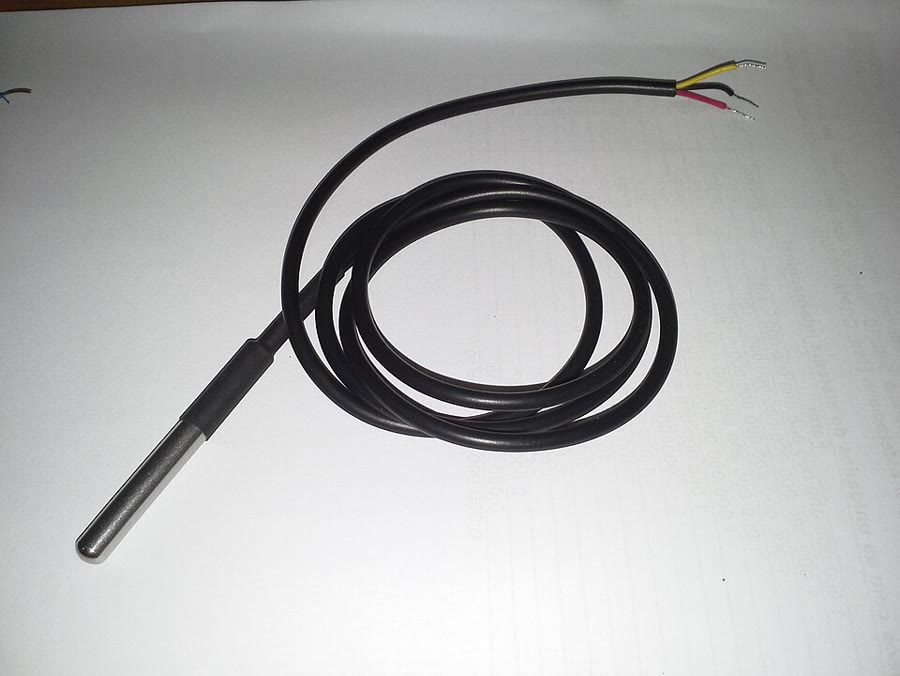
\includegraphics[width=0.45\linewidth]{images/book2/g10-temperature-sensor.jpg}

{\small A temperature \omterm{def:g10:sensors-actuators-control:sensor}{sensor} sealed in a steel tube at the end of its cable, ready to be dipped in water or buried
in a wall; the computer at the other end reads its temperature as a number. Photograph: Leonardo Postay,
CC BY-SA 4.0.}
\end{omfigure}

\begin{definition}[Control loop]\label{def:g10:sensors-actuators-control:control-loop}
A \emph{control loop}\index{control loop} is the loop that an embedded program repeats for as long as the object
runs: read the \omterm{def:g10:sensors-actuators-control:sensor}{sensors}, decide, command the \omterm{def:g10:sensors-actuators-control:sensor}{actuators}, wait until the next period.
\end{definition}

\begin{omfigure}
\begin{tikzpicture}[font=\footnotesize, node distance=14mm, b/.style={draw, rounded corners=2pt, minimum height=9mm,
    minimum width=22mm, align=center}]
  \node[b, fill=omDef!8] (s) {sensor\\(thermometer)};
  \node[b, fill=omCode!8, right=of s] (c) {program\\read, decide, act};
  \node[b, fill=omProp!10, right=of c] (a) {actuator\\(heater)};
  \node[b, below=10mm of c, minimum width=60mm, fill=omMeth!8] (w) {the room};
  \draw[ptr] (s) -- node[above] {number} (c);
  \draw[ptr] (c) -- node[above] {on / off} (a);
  \draw[ptr, omProp] (a) |- node[pos=0.25, right] {heat} (w);
  \draw[ptr, omMeth] (w) -| node[pos=0.75, left] {temperature} (s);
\end{tikzpicture}

{\small The \omterm{def:g10:sensors-actuators-control:control-loop}{control loop} of a thermostat. The program never sees the room, only numbers; its decisions change the
room, which changes the next numbers.}
\end{omfigure}

\section{Measured values turned into numbers}\label{sec:g10:sensors-actuators-control:values}

The simulated thermometer of the chapter gives a whole number from $0$ to $1023$, on $10$ bits, where $0$ means
$-20$~°C and $1023$ means $60$~°C. Turning it into degrees takes an offset and a scale.

\omcode{code/grade-10/10-sensors-actuators-control/listings/convert.py}{1}{12}{From a $10$-bit reading to
degrees.}\label{lst:g10:sensors-actuators-control:convert}

\omoutput{code/grade-10/10-sensors-actuators-control/outputs/convert.txt}{A step of the reading is
$80/1023 \approx 0.078$ degree: the \omterm{def:g10:sensors-actuators-control:sensor}{sensor} cannot tell apart two temperatures closer than
that.}\label{out:g10:sensors-actuators-control:convert}

A real measurement also wobbles from one reading to the next: electrical noise, air moving past the \omterm{def:g10:sensors-actuators-control:sensor}{sensor}. The
simulated \omterm{def:g10:sensors-actuators-control:sensor}{sensor} adds a random error of about $0.3$ degree. Averaging the last few readings smooths it out, at the
price of reacting a little later.

\omcode{code/grade-10/10-sensors-actuators-control/listings/smooth.py}{1}{19}{A moving average of five
readings.}\label{lst:g10:sensors-actuators-control:smooth}

\omoutput{code/grade-10/10-sensors-actuators-control/outputs/smooth.txt}{The true value is $20.0$~°C: averaging
divides the spread of the readings by almost three.}\label{out:g10:sensors-actuators-control:smooth}

The simplest thermostat switches the heater on below the target and off above it. With noisy readings near the
target, it flips the heater on and off at every reading, which wears the switch out.

\begin{definition}[Hysteresis]\label{def:g10:sensors-actuators-control:hysteresis}
A controller with \emph{hysteresis}\index{hysteresis} uses two thresholds instead of one: it switches on below the
lower one and off above the higher one, and between them it keeps its current \omterm{def:g10:sensors-actuators-control:state-machine}{state}. The gap between the two
thresholds is the \emph{band}.
\end{definition}

\omcode{code/grade-10/10-sensors-actuators-control/listings/thermostat.py}{1}{30}{Two thermostats for the same
room.}\label{lst:g10:sensors-actuators-control:thermostat}

\omoutput{code/grade-10/10-sensors-actuators-control/outputs/thermostat.txt}{Six simulated hours: the band of one
degree cuts the switching by almost three, for a temperature that moves a little
more.}\label{out:g10:sensors-actuators-control:thermostat}

The function \code{room} of the chapter's \code{sensor.py} simulates the room minute by minute: it loses heat towards
the $8$~°C outside, gains heat when the heater is on, and asks the controller each minute what to do with a fresh
noisy reading.

\begin{omfigure}
\begin{tikzpicture}
  \begin{axis}[omrecord, width=0.9\linewidth, height=5.2cm, xlabel={minute}, ylabel={temperature (°C)},
      xmin=120, xmax=240, ymin=18.6, ymax=21.1, legend pos=south east, legend cell align=left,
      legend style={fill=white, fill opacity=0.9}]
    \addplot[omThm, thin, const plot] table[x=minute, y=plain]
      {code/grade-10/10-sensors-actuators-control/figures/thermostat_plot.dat};
    \addlegendentry{plain on/off at 20}
    \addplot[omDef, thick, const plot] table[x=minute, y=hyst]
      {code/grade-10/10-sensors-actuators-control/figures/thermostat_plot.dat};
    \addlegendentry{hysteresis, 19.5 to 20.5}
    \addplot[black!40, dashed, domain=120:240] {19.5};
    \addplot[black!40, dashed, domain=120:240] {20.5};
  \end{axis}
\end{tikzpicture}

{\small Two hours of the simulated room. The plain thermostat keeps the temperature close to $20$ but switches
almost every minute; with \omterm{def:g10:sensors-actuators-control:hysteresis}{hysteresis} the temperature rises and falls through the band in long, regular swings.}
\end{omfigure}

\section{A controller as a state machine}\label{sec:g10:sensors-actuators-control:machines}

A thermostat has two \omterm{def:g10:sensors-actuators-control:state-machine}{states}, heating or not. A traffic light or a lift has more, and what it does with an \omterm{def:g10:sensors-actuators-control:state-machine}{event}, a
button pressed, a floor reached, depends on the \omterm{def:g10:sensors-actuators-control:state-machine}{state} it is in.

\begin{omfigure}
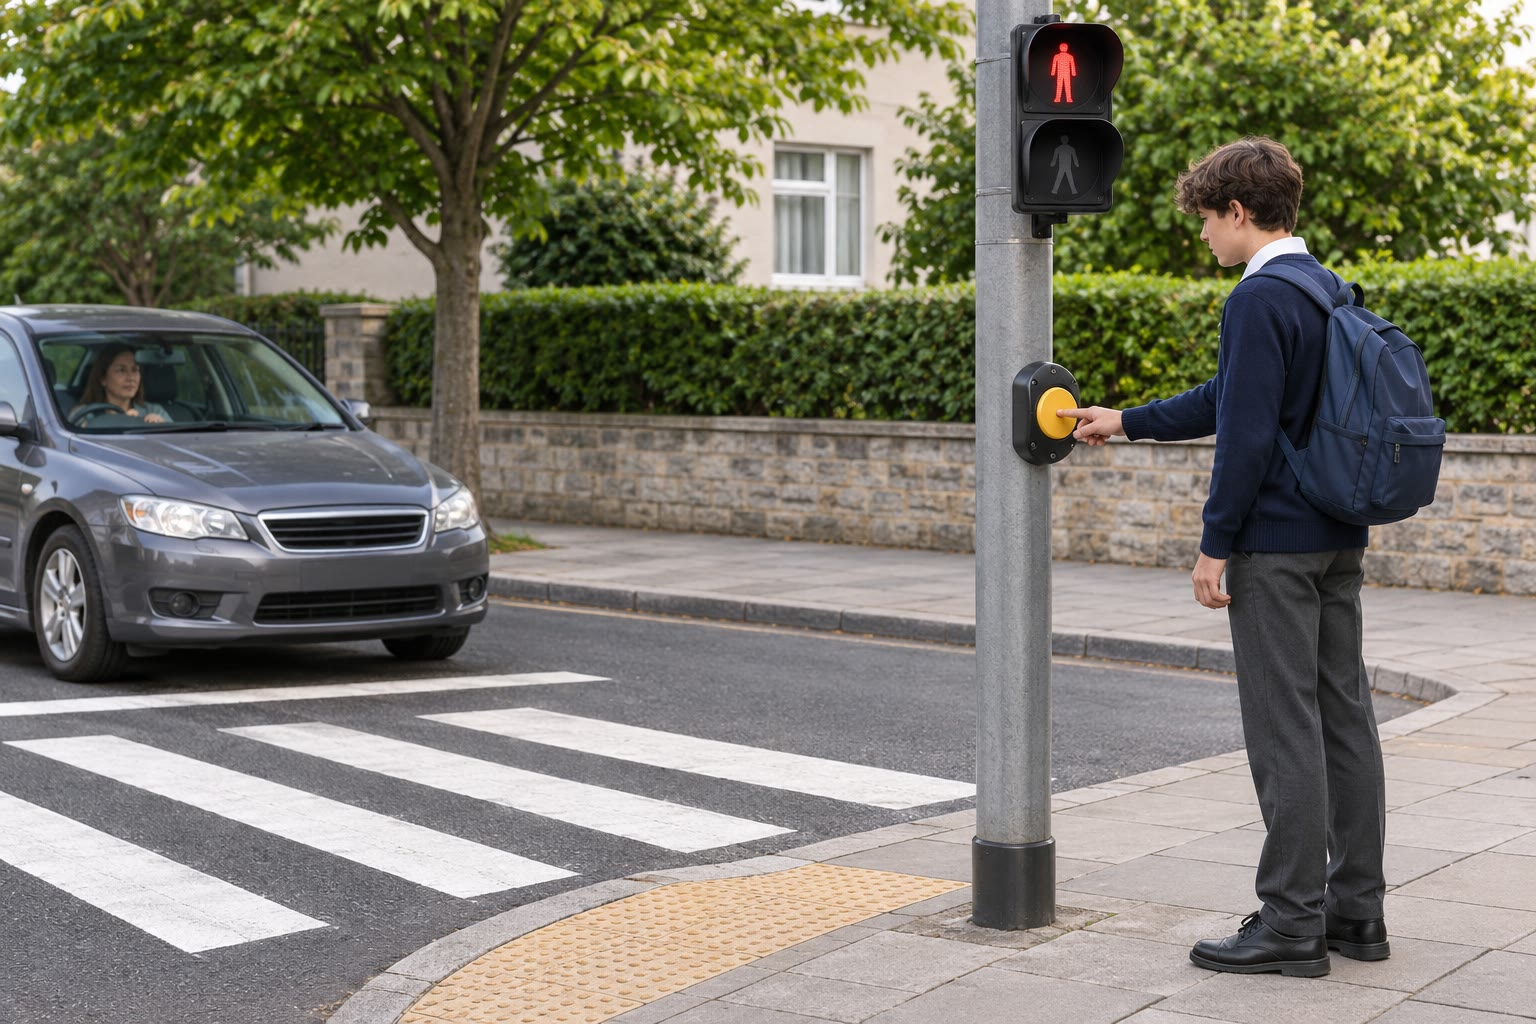
\includegraphics[width=0.55\linewidth]{images/book2/ai/g10-sensors-actuators-control-crossing.jpg}

{\small A pedestrian crossing with its button: pressing it is an \omterm{def:g10:sensors-actuators-control:state-machine}{event}, and what the light does next depends on its \omterm{def:g10:sensors-actuators-control:state-machine}{state}.}
\end{omfigure}

\begin{definition}[State machine]\label{def:g10:sensors-actuators-control:state-machine}
A \emph{state machine}\index{state machine} is made of a set of \emph{states}\index{state}, one of which is the
current one, a set of \emph{events}\index{event}, and \emph{transitions}\index{transition}: for a state and an
event, the next state. The machine starts in an initial state, and each event moves it along one transition.
\end{definition}

A \omterm{def:g10:sensors-actuators-control:state-machine}{transition} table is a dictionary from (\omterm{def:g10:sensors-actuators-control:state-machine}{state}, \omterm{def:g10:sensors-actuators-control:state-machine}{event}) to the next \omterm{def:g10:sensors-actuators-control:state-machine}{state}. Here is the light that the cars see at a
pedestrian crossing: a press on the button does not stop the cars at once, it schedules a red light.

\begin{omfigure}
\begin{tikzpicture}[->, >={Stealth[length=2mm]}, node distance=30mm, font=\footnotesize,
    every state/.style={draw, minimum size=14mm, align=center, font=\footnotesize}]
  \node[state, initial, initial text={}, fill=omMeth!15] (g) {green};
  \node[state, right=of g, fill=omMeth!15] (w) {green\\wait};
  \node[state, right=of w, fill=ocYellow!40] (a) {amber};
  \node[state, below=16mm of w, fill=omThm!20] (r) {red};
  \path (g) edge node[above] {button} (w)
        (w) edge node[above] {tick} (a)
        (a) edge[bend left=20] node[below right] {tick} (r)
        (r) edge[bend left=20] node[below left] {tick} (g)
        (g) edge[loop above] node {tick} ()
        (w) edge[loop above] node {button} ();
\end{tikzpicture}

{\small The crossing as a \omterm{def:g10:sensors-actuators-control:state-machine}{state machine}. A \textit{tick} is the end of a timed period. The pairs not drawn, such as
amber with \textit{button}, leave the \omterm{def:g10:sensors-actuators-control:state-machine}{state} unchanged.}
\end{omfigure}

\omcode{code/grade-10/10-sensors-actuators-control/listings/traffic_light.py}{1}{19}{A table-driven traffic
light.}\label{lst:g10:sensors-actuators-control:traffic-light}

\omoutput{code/grade-10/10-sensors-actuators-control/outputs/traffic_light.txt}{A trace of seven \omterm{def:g10:sensors-actuators-control:state-machine}{events}. The second
press changes nothing: a red light is already on its way.}\label{out:g10:sensors-actuators-control:traffic-light}

\begin{method}[Writing a controller as a state machine]\label{met:g10:sensors-actuators-control:method}
\begin{enumerate}
  \item List the \omterm{def:g10:sensors-actuators-control:state-machine}{states}, and say what each \omterm{def:g10:sensors-actuators-control:sensor}{actuator} does in each of them.
  \item List the \omterm{def:g10:sensors-actuators-control:state-machine}{events}: readings that cross a threshold, buttons, timers.
  \item For every pair (\omterm{def:g10:sensors-actuators-control:state-machine}{state}, \omterm{def:g10:sensors-actuators-control:state-machine}{event}), decide the next \omterm{def:g10:sensors-actuators-control:state-machine}{state}, including ``no change''; a table must have no hole.
  \item Write the property that must never fail, as a test on a \omterm{def:g10:sensors-actuators-control:state-machine}{state}, and check it on every \omterm{def:g10:sensors-actuators-control:state-machine}{state} the machine can
    reach.
\end{enumerate}
\end{method}

\section{The lift}\label{sec:g10:sensors-actuators-control:lift}

The lift of the town hall serves floors $0$, $1$ and $2$. Its \omterm{def:g10:sensors-actuators-control:state-machine}{state} is a tuple: the floor, the door (open or closed),
the motor (stopped, going up, going down) and the floor it is going to. Its \omterm{def:g10:sensors-actuators-control:state-machine}{events} are a call to a floor, a request
to open or close the door, and the signal \textit{arrive} that a \omterm{def:g10:sensors-actuators-control:sensor}{sensor} in the shaft sends when the cabin reaches a
floor. The rules are written as a function instead of a table: there are many \omterm{def:g10:sensors-actuators-control:state-machine}{states}, but few kinds of rules.

\omcode{code/grade-10/10-sensors-actuators-control/listings/lift.py}{1}{32}{The lift's \omterm{def:g10:sensors-actuators-control:state-machine}{transitions}, and the safety
property.}\label{lst:g10:sensors-actuators-control:lift}

\omoutput{code/grade-10/10-sensors-actuators-control/outputs/lift.txt}{The first call is refused while the door is
open, and the request to open is refused while the cabin moves.}\label{out:g10:sensors-actuators-control:lift}

\begin{omfigure}
\begin{tikzpicture}[->, >={Stealth[length=2mm]}, font=\scriptsize, x=36mm, y=24mm,
    every state/.style={draw, minimum size=11mm, align=center, font=\scriptsize}]
  \foreach \f in {0,1,2} {
    \node[state] (c\f) at (\f,2) {floor \f\\closed};
    \node[state, fill=omMeth!15] (o\f) at (\f,0) {floor \f\\open};
    \path (c\f) edge[bend right=12] (o\f)
          (o\f) edge[bend right=12] (c\f);
  }
  \node[state, fill=omProp!15] (u) at (0.5,1) {moving\\up};
  \node[state, fill=omProp!15] (d) at (1.5,1) {moving\\down};
  \begin{scope}[omDef, thick, every node/.style={sloped, fill=white, inner sep=1pt, pos=0.45}]
    \draw (c0) -- node {call 1, 2} (u);
    \draw (c1) -- node {call 2} (u);
    \draw (c1) -- node {call 0} (d);
    \draw (c2) -- node {call 0, 1} (d);
  \end{scope}
  \begin{scope}[omProp, thick]
    \draw (u) -- (o1);
    \draw (u) -- (o2);
    \draw (d) -- (o1);
    \draw (d) -- (o0);
  \end{scope}
\end{tikzpicture}

{\small The lift's \omterm{def:g10:sensors-actuators-control:state-machine}{states}. Each moving \omterm{def:g10:sensors-actuators-control:state-machine}{state} stands for three \omterm{def:g10:sensors-actuators-control:state-machine}{states}, with their floor and target; the orange
arrows are \textit{arrive} at the target, which stops the motor and opens the door in one \omterm{def:g10:sensors-actuators-control:state-machine}{transition}; the black arrows
are \textit{open} (downwards) and \textit{close} (upwards). Calls start the motor only from a closed \omterm{def:g10:sensors-actuators-control:state-machine}{state}.}
\end{omfigure}

A person does not send \omterm{def:g10:sensors-actuators-control:state-machine}{events} by hand; a panel of buttons does. A small text interface plays the panel: it reads a
command, checks it, sends the \omterm{def:g10:sensors-actuators-control:state-machine}{event} and shows the new \omterm{def:g10:sensors-actuators-control:state-machine}{state}.

\omcode{code/grade-10/10-sensors-actuators-control/listings/lift_menu.py}{1}{15}{A text panel for the
lift.}\label{lst:g10:sensors-actuators-control:lift-menu}

\omoutput{code/grade-10/10-sensors-actuators-control/outputs/lift_menu.txt}{A session: typing errors are refused,
and every \omterm{def:g10:sensors-actuators-control:state-machine}{state} reached is checked.}\label{out:g10:sensors-actuators-control:lift-menu}

Checking the \omterm{def:g10:sensors-actuators-control:state-machine}{states} of a few sessions shows that the lift was safe in those sessions. To be sure for every session,
the weekend problem checks every \omterm{def:g10:sensors-actuators-control:state-machine}{state} the lift can ever reach: there are few of them, so all can be listed.

\begin{safety}
Never test a control program on the real device first. Simulate it, check its \omterm{def:g10:sensors-actuators-control:state-machine}{states}, then try it on the device
with the power limited and a person at the emergency switch. Real lifts, machines and vehicles also have safety
devices that do not depend on the program: a door contact that cuts the motor's power whatever the computer says.
\end{safety}

\section{Exercises}\label{sec:g10:sensors-actuators-control:exercises}

\begin{exercise}[$\star$]\label{exo:g10:sensors-actuators-control:1}
The \omterm{def:g10:sensors-actuators-control:sensor}{sensor} reads $300$, then $700$. Convert both to degrees. Which reading corresponds to $0$~°C most closely?
\end{exercise}

\begin{exercise}[$\star$]\label{exo:g10:sensors-actuators-control:2}
In the traffic light's table, what is the next \omterm{def:g10:sensors-actuators-control:state-machine}{state} of \textit{amber} on \textit{button}, and of \textit{red} on
\textit{tick}? Starting from \textit{green}, which \omterm{def:g10:sensors-actuators-control:state-machine}{events} lead to \textit{red} fastest?
\end{exercise}

\begin{exercise}[$\star$]\label{exo:g10:sensors-actuators-control:3}
Compute by hand the moving averages of width $5$ of the readings $20.1$, $19.7$, $20.4$, $19.9$, $20.3$, $19.6$,
$20.0$.
\end{exercise}

\begin{exercise}[$\star$]\label{exo:g10:sensors-actuators-control:4}
A machine has $6$ \omterm{def:g10:sensors-actuators-control:state-machine}{states} and $4$ \omterm{def:g10:sensors-actuators-control:state-machine}{events}. How many entries does a complete \omterm{def:g10:sensors-actuators-control:state-machine}{transition} table have? How many does the
traffic light's table have, and is it complete?
\end{exercise}

\begin{exercise}[$\star$]\label{exo:g10:sensors-actuators-control:5}
Write \code{to_celsius(raw)} for a \omterm{def:g10:sensors-actuators-control:sensor}{sensor} whose $10$-bit readings span $-40$~°C to $85$~°C. What is its step?
\end{exercise}

\begin{exercise}[$\star\star$]\label{exo:g10:sensors-actuators-control:6}
A student removes the line \code{("amber", "button"): "amber"} from the table, and a pedestrian presses the button
during the amber light. What happens to the program, and why is it dangerous in a real crossing? Write a
\code{next_state(table, state, event)} that cannot fail this way.
\end{exercise}

\begin{exercise}[$\star\star$]\label{exo:g10:sensors-actuators-control:7}
Write a thermostat for a greenhouse to this specification: the heater goes on when the temperature falls below
$18$~°C, off when it rises above $21$~°C, and keeps its \omterm{def:g10:sensors-actuators-control:state-machine}{state} in between.
\end{exercise}

\begin{exercise}[$\star\star$]\label{exo:g10:sensors-actuators-control:8}
The readings are $19.6$, $19.4$, $19.6$, $19.3$, $19.7$, $17.8$, $19.8$, $21.2$, $19.4$, $19.6$, and the heater is
off at the start. How many times does a plain thermostat at $19.5$ switch? And the greenhouse thermostat of the
previous exercise?
\end{exercise}

\begin{exercise}[$\star\star$]\label{exo:g10:sensors-actuators-control:9}
Give the trace of the traffic light, from \textit{green}, for the \omterm{def:g10:sensors-actuators-control:state-machine}{events} \textit{button}, \textit{tick},
\textit{button}, \textit{tick}, \textit{tick}, \textit{button}, \textit{tick}. How many ticks do cars wait at red?
\end{exercise}

\begin{exercise}[$\star\star$]\label{exo:g10:sensors-actuators-control:10}
A new version of the lift accepts a call whenever the motor is stopped, without looking at the door. Starting with
the door open at floor $0$, which \omterm{def:g10:sensors-actuators-control:state-machine}{event} leads to an unsafe \omterm{def:g10:sensors-actuators-control:state-machine}{state}? Show it with the function \code{safe}.
\end{exercise}

\begin{exercise}[$\star\star$]\label{exo:g10:sensors-actuators-control:11}
Write \code{check_safe(states, events, step, safe)}, which returns every pair (\omterm{def:g10:sensors-actuators-control:state-machine}{state}, \omterm{def:g10:sensors-actuators-control:state-machine}{event}) that leads from a safe
\omterm{def:g10:sensors-actuators-control:state-machine}{state} to an unsafe one. Run it on the lift and on the version of the previous exercise.
\end{exercise}

\begin{exercise}[$\star\star\star$]\label{exo:g10:sensors-actuators-control:12}
Prove that a thermostat with \omterm{def:g10:sensors-actuators-control:hysteresis}{hysteresis}, thresholds $a < b$, switches on only when the reading is below $a$, and
switches off only when it is above $b$. Deduce that between two switchings on, the readings have gone above $b$
once: the heater switches at most once each time the readings cross the whole band.
\end{exercise}

\begin{exercise}[$\star\star\star$]\label{exo:g10:sensors-actuators-control:13}
A car park with $3$ spaces has a barrier at the entry. Its controller counts the cars inside: it lets a car in only
if there is room, and counts it out when it leaves. Write it as a function \code{barrier(state, event)} and test it
with four cars arriving and one leaving.
\end{exercise}

\begin{exercise}[$\star\star\star$]\label{exo:g10:sensors-actuators-control:14}
A smaller lift serves only floors $0$ and $1$. List by hand all its reachable \omterm{def:g10:sensors-actuators-control:state-machine}{states}, starting from floor $0$ with the
door closed, and check the safety property on each.
\end{exercise}

\begin{exercise}[$\star\star\star$]\label{exo:g10:sensors-actuators-control:15}
A \omterm{def:g10:sensors-actuators-control:control-loop}{control loop} reads a command with \code{input()} at each turn, then reads the thermometer and drives the heater.
What happens to the heating while nobody types anything? Propose a structure in which the loop never waits for a
person.
\end{exercise}

\section{Problem: The Lift of the Town Hall}\label{sec:g10:sensors-actuators-control:problem}

\begin{problem}[{Weekend problem --- proving the lift safe by checking every state}]\label{pb:g10:sensors-actuators-control:1}
The program \code{exercises/lift_check.py} starts from floor $0$ with the door closed, tries every \omterm{def:g10:sensors-actuators-control:state-machine}{event} in every
\omterm{def:g10:sensors-actuators-control:state-machine}{state} it finds, and stops when no new \omterm{def:g10:sensors-actuators-control:state-machine}{state} appears. It then serves a list of calls and counts the \omterm{def:g10:sensors-actuators-control:state-machine}{events} each one
needs.

\medskip\noindent\textbf{Part I --- States and events.}
\begin{enumerate}
  \item How many values can each of the four parts of the lift's \omterm{def:g10:sensors-actuators-control:state-machine}{state} take? How many tuples is that at most?
  \item List the six \omterm{def:g10:sensors-actuators-control:state-machine}{events}.
  \item Why can the target be \code{None}, and when is it?
  \item Which \omterm{def:g10:sensors-actuators-control:state-machine}{states}, among those tuples, would be unsafe?
\end{enumerate}

\medskip\noindent\textbf{Part II --- The transitions.}
\begin{enumerate}[resume]
  \item From $(0, \text{closed}, \text{stop}, \text{None})$, give the next \omterm{def:g10:sensors-actuators-control:state-machine}{state} for each of the six \omterm{def:g10:sensors-actuators-control:state-machine}{events}.
  \item From $(1, \text{closed}, \text{up}, 2)$, give the next \omterm{def:g10:sensors-actuators-control:state-machine}{state} for each of the six \omterm{def:g10:sensors-actuators-control:state-machine}{events}.
  \item Which \omterm{def:g10:sensors-actuators-control:state-machine}{transitions} open the door? Check that each leaves the motor stopped.
  \item Which \omterm{def:g10:sensors-actuators-control:state-machine}{transitions} start the motor? Check that each requires the door closed.
\end{enumerate}

\medskip\noindent\textbf{Part III --- Every reachable state.}
\begin{enumerate}[resume]
  \item Run the program. How many \omterm{def:g10:sensors-actuators-control:state-machine}{states} are reachable?
  \item List them: the stopped ones, then the moving ones with their targets.
  \item Why is $(1, \text{closed}, \text{up}, 1)$ never reached?
  \item The program finds no unsafe \omterm{def:g10:sensors-actuators-control:state-machine}{state}. Why does that prove that the lift is never unsafe, whatever \omterm{def:g10:sensors-actuators-control:state-machine}{events}
    arrive, in whatever order?
  \item Does the proof still hold if the lift starts with its door open at floor $0$?
\end{enumerate}

\medskip\noindent\textbf{Part IV --- Serving calls.}
\begin{enumerate}[resume]
  \item For the calls $2$, $0$, $1$, $2$, $1$, the program counts the \omterm{def:g10:sensors-actuators-control:state-machine}{events} each needs. Explain the $3$ and the $4$.
  \item What is the mean number of \omterm{def:g10:sensors-actuators-control:state-machine}{events} per call?
  \item Find a list of five calls with a larger mean, and one with a smaller mean.
  \item A real lift would serve a call at floor $1$ on its way from $0$ to $2$. Which part of the \omterm{def:g10:sensors-actuators-control:state-machine}{state} would that
    change?
  \item Why would checking every \omterm{def:g10:sensors-actuators-control:state-machine}{state} be harder for a lift of $20$ floors, and still possible?
  \item \omterm{def:g10:sensors-actuators-control:state-machine}{State} the result: the number of reachable \omterm{def:g10:sensors-actuators-control:state-machine}{states}, and why the door is never open while the cabin moves.
\end{enumerate}
\end{problem}
